\documentclass[12pt]{article}
 
\usepackage[margin=1in]{geometry} 
\usepackage{amsmath,amsthm,amssymb}

\usepackage[brazilian]{babel}
\usepackage[utf8]{inputenc}
\usepackage[T1]{fontenc}
\usepackage{graphicx}         %pacote para incluir figuras tipo eps
\usepackage{xcolor}
\usepackage{float} 
\usepackage{epstopdf}
\usepackage{longtable}
 
 %Matlab code in latex 
\usepackage[final]{listings}
\usepackage{color} %red, green, blue, yellow, cyan, magenta, black, white
\definecolor{mygreen}{RGB}{28,172,0}
\definecolor{mylilas}{RGB}{170,55,241}
\lstdefinestyle{myMatlab}
{
language=matlab,frame=single, basicstyle=\small\ttfamily,breaklines=true,%
morekeywords={matlab2tikz}, keywordstyle=\color{blue}, morekeywords=[2]{1}, keywordstyle=[2]{\color{black}}, commentstyle=\color{mygreen}, stringstyle=\color{mylilas}, identifierstyle=\color{black}, showstringspaces=false,%without this there will be a symbol in the places where there is a space
numbers=left, numberstyle={\scriptsize \color{black}},% size of the numbers
numbersep=9pt, % this defines how far the numbers are from the text
% emph=[1]{for,end,break},emphstyle=[1]\color{red}, %some words to emphasise
% emph=[2]{word1,word2}, emphstyle=[2]{style},
}
 
\newcommand{\N}{\mathbb{N}}
\newcommand{\Z}{\mathbb{Z}}
 
\newenvironment{theorem}[2][Theorem]{\begin{trivlist}
\item[\hskip \labelsep {\bfseries #1}\hskip \labelsep {\bfseries #2.}]}{\end{trivlist}}
\newenvironment{lemma}[2][Lemma]{\begin{trivlist}
\item[\hskip \labelsep {\bfseries #1}\hskip \labelsep {\bfseries #2.}]}{\end{trivlist}}
\newenvironment{exercise}[2][Exercício]{\begin{trivlist}
\item[\hskip \labelsep {\bfseries #1}\hskip \labelsep {\bfseries #2.}]}{\end{trivlist}}
\newenvironment{reflection}[2][Reflection]{\begin{trivlist}
\item[\hskip \labelsep {\bfseries #1}\hskip \labelsep {\bfseries #2.}]}{\end{trivlist}}
\newenvironment{proposition}[2][Proposition]{\begin{trivlist}
\item[\hskip \labelsep {\bfseries #1}\hskip \labelsep {\bfseries #2.}]}{\end{trivlist}}
\newenvironment{corollary}[2][Corollary]{\begin{trivlist}
\item[\hskip \labelsep {\bfseries #1}\hskip \labelsep {\bfseries #2.}]}{\end{trivlist}}
 
\begin{document}
 
% --------------------------------------------------------------
%                         Start here
% --------------------------------------------------------------
 
\title{Exercício 02}
\author{Renan Salles de Freitas\\
CPE 723 - Otimização Natural}
 
\maketitle
 
\begin{exercise}{1.a}
Temos que a distribuição de probabilidade de $X(1)$ é:
\begin{align*}
\textbf{p}_1 &= M\textbf{p}_0
\end{align*}
E ainda:
\begin{align*}
\textbf{p}_2 = M\textbf{p}_1 &= M^2\textbf{p}_0 \\
\textbf{p}_n &= M^n\textbf{p}_0
\end{align*}
Portanto:
\begin{align*}
\textbf{p}_3 &= M^3\textbf{p}_0 \\
\textbf{p}_3 &= \begin{bmatrix}
0.3328 \\ 0.3344 \\ 0.3328
\end{bmatrix}
\end{align*}
\end{exercise}
 
\begin{exercise}{1.b} Supondo que estamos no estado $X(t)$, construímos uma
lista com os possíveis próximos estados, considerando a distribuição de
probabilidade, conforme a matriz de transição de estados $M$:
$X(t+1) = [X(t) \quad 0 \quad 1 \quad 2]$. Sorteamos um índice de zero a quatro
com o MatLab e atualizamos $X(t+1)$. Observe que, dessa forma, a transsição
para o estado o estado atual sempre possui probabilidade $0.5$ e os outros
estados possuem probabilidade $0.25$.
\begin{align}
X(0) &= 1 \\
\nonumber \text{list} &= [0 \quad 1 \quad 2 \quad 1] \\
\nonumber r &= \text{randi}(4) = 3 \\
\nonumber X(1) &= \text{list}(r) = 2  
\end{align}

\begin{align}
X(1) &= 2 \\
\nonumber \text{list} &= [0 \quad 1 \quad 2 \quad 2] \\
\nonumber r &= \text{randi}(4) = 3 \\
\nonumber X(2) &= \text{list}(r) = 2  
\end{align}

\begin{align}
X(2) &= 2 \\
\nonumber \text{list} &= [0 \quad 1 \quad 2 \quad 2] \\
\nonumber r &= \text{randi}(4) = 4 \\
\nonumber X(3) &= \text{list}(r) = 2  
\end{align}

\end{exercise}

\begin{exercise}{1.c} Código MatLab abaixo:
\lstinputlisting[style=myMatlab]{matlab/ex1_c.m} 

%\begin{table}[]
%\centering
\begin{longtable}{cccc} $\textbf{X(0)}$ & $\textbf{X(1)}$ & $\textbf{X(2)}$ &
$\textbf{X(3)}$\\ \endfirsthead $\textbf{X(0)}$ & $\textbf{X(1)}$ & $\textbf{X(2)}$ &
$\textbf{X(3)}$\\
\endhead
2      & 2      & 2      & 1      \\
2      & 2      & 0      & 0      \\
2      & 0      & 0      & 2      \\
2      & 0      & 2      & 0      \\
1      & 1      & 1      & 1      \\
1      & 1      & 2      & 0      \\
2      & 2      & 2      & 2      \\
0      & 1      & 0      & 0      \\
0      & 0      & 1      & 1      \\
1      & 2      & 2      & 2      \\
1      & 0      & 0      & 0      \\
2      & 1      & 1      & 1      \\
2      & 2      & 1      & 2      \\
1      & 0      & 2      & 0      \\
1      & 0      & 2      & 0      \\
2      & 0      & 0      & 2      \\
0      & 2      & 0      & 0      \\
1      & 0      & 0      & 1      \\
1      & 1      & 1      & 1      \\
1      & 1      & 1      & 2      \\
0      & 0      & 1      & 2      \\
2      & 0      & 0      & 2      \\
0      & 0      & 0      & 1      \\
1      & 1      & 2      & 2      \\
0      & 1      & 0      & 2      \\
0      & 2      & 2      & 2      \\
2      & 1      & 0      & 0      \\
1      & 1      & 1      & 2      \\
2      & 0      & 1      & 0      \\
2      & 2      & 1      & 1      \\
2      & 2      & 2      & 0      \\
0      & 0      & 0      & 2      \\
2      & 2      & 1      & 0      \\
0      & 0      & 0      & 1      \\
1      & 0      & 2      & 0      \\
1      & 2      & 1      & 2      \\
1      & 1      & 1      & 0      \\
1      & 0      & 2      & 2      \\
0      & 1      & 1      & 1      \\
1      & 2      & 2      & 1      \\
2      & 0      & 2      & 0      \\
1      & 0      & 1      & 1      \\
2      & 0      & 2      & 2      \\
1      & 0      & 1      & 1      \\
2      & 0      & 0      & 1      \\
2      & 2      & 0      & 2      \\
1      & 2      & 0      & 1      \\
2      & 1      & 0      & 0      \\
1      & 0      & 0      & 1      \\
0      & 0      & 0      & 2      \\
0      & 1      & 1      & 0      \\
2      & 2      & 1      & 2      \\
2      & 2      & 2      & 0      \\
2      & 2      & 2      & 0      \\
2      & 1      & 0      & 0      \\
1      & 2      & 1      & 1      \\
2      & 0      & 2      & 1      \\
1      & 1      & 2      & 1      \\
2      & 2      & 2      & 2      \\
2      & 1      & 0      & 0      \\
2      & 2      & 2      & 2      \\
2      & 1      & 0      & 1      \\
0      & 2      & 2      & 2      \\
2      & 2      & 0      & 1      \\
2      & 2      & 0      & 0      \\
1      & 1      & 2      & 0      \\
0      & 1      & 1      & 1      \\
1      & 1      & 1      & 1      \\
0      & 0      & 0      & 1      \\
0      & 0      & 0      & 0      \\
0      & 2      & 2      & 2      \\
2      & 1      & 1      & 1      \\
2      & 2      & 2      & 2      \\
1      & 0      & 2      & 2      \\
0      & 0      & 0      & 2      \\
2      & 2      & 2      & 2      \\
2      & 0      & 1      & 1      \\
1      & 1      & 2      & 1      \\
1      & 0      & 0      & 0      \\
1      & 1      & 1      & 2      \\
0      & 1      & 1      & 0      \\
0      & 0      & 1      & 1      \\
1      & 1      & 2      & 2      \\
0      & 0      & 0      & 0      \\
1      & 1      & 0      & 0      \\
1      & 2      & 1      & 1      \\
0      & 0      & 1      & 2      \\
0      & 2      & 2      & 1      \\
1      & 1      & 1      & 0      \\
0      & 2      & 0      & 0      \\
1      & 0      & 2      & 2      \\
1      & 1      & 2      & 0      \\
1      & 0      & 0      & 0      \\
2      & 0      & 0      & 0      \\
1      & 2      & 1      & 2      \\
1      & 2      & 2      & 2      \\
0      & 0      & 0      & 2      \\
2      & 0      & 1      & 1      \\
2      & 1      & 1      & 1      \\
1      & 0      & 0      & 0     
\end{longtable}
\end{exercise}

\begin{exercise}{1.d} Os hisstogramas estão representados abaixo:
\begin{figure}[H]
  \centering
  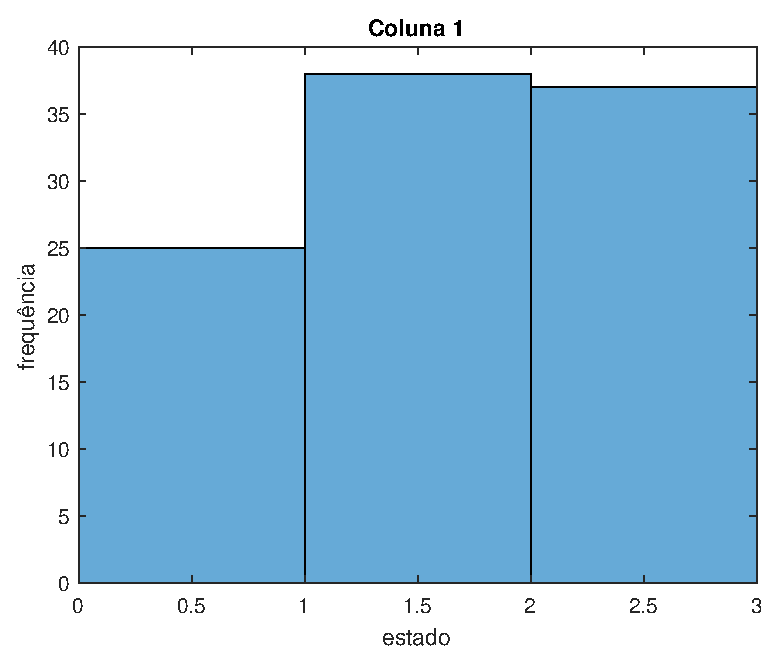
\includegraphics[width=8cm]{figs/ex1_1.eps} 
\end{figure}
\begin{figure}[H]
  \centering
  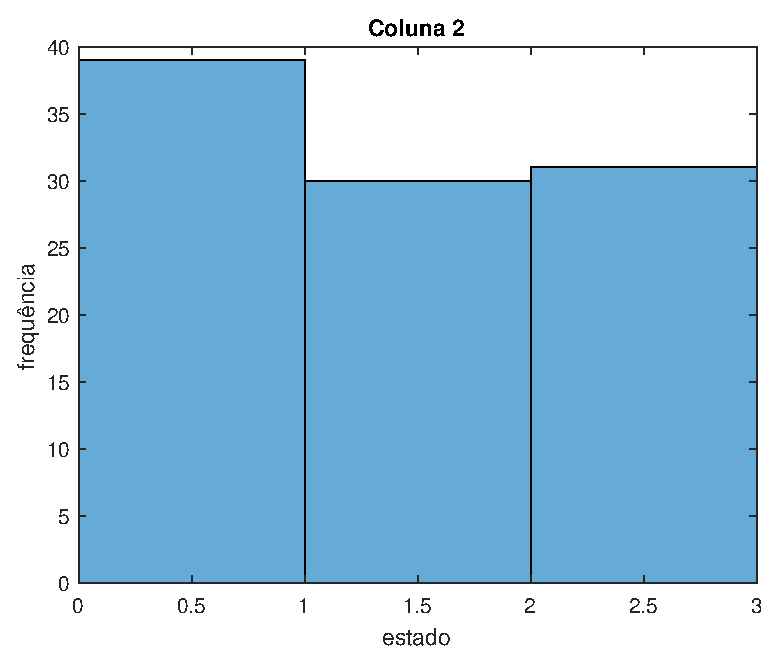
\includegraphics[width=8cm]{figs/ex1_2.eps} 
\end{figure}
\begin{figure}[H]
  \centering
  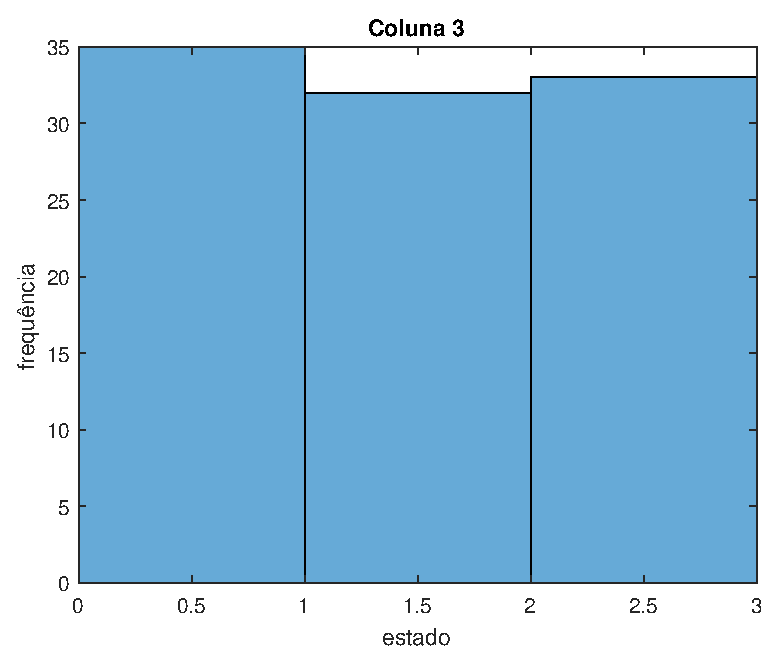
\includegraphics[width=8cm]{figs/ex1_3.eps} 
\end{figure}
\begin{figure}[H]
  \centering
  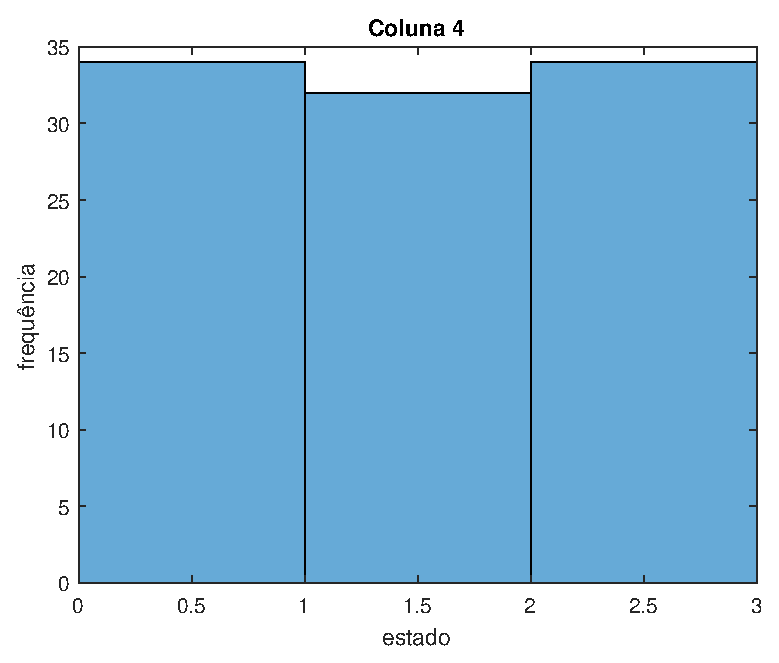
\includegraphics[width=8cm]{figs/ex1_4.eps} 
\end{figure}

O código MatLab para calcualr as proobabilidades está abaixo:
\lstinputlisting[style=myMatlab]{matlab/ex1_d2.m}

Sabemos que o estado inicial é equiprovável para os três estados :
\begin{align*}
\textbf{p}_0 &= [0.3333 \quad 0.3333 \quad 0.3333]
\end{align*} 
E ainda:
\begin{align*}
\textbf{p}_1 &= M\textbf{p}_0 = [0.3333 \quad 0.3333 \quad
0.3333] \\
\textbf{p}_n &= M^n\textbf{p}_0 = \textbf{p}_0 = [0.3333 \quad 0.3333 \quad
0.3333]
\end{align*}

Calculamos as probabilidades pela frequência do histograma e obtemos:
\begin{align*}
\textbf{p}_0 &= [0.25 \quad 0.38 \quad 0.37]
\textbf{p}_1 &= [0.39 \quad 0.30 \quad 0.31]
\textbf{p}_2 &= [0.35 \quad 0.32 \quad 0.33]
\textbf{p}_3 &= [0.34 \quad 0.32 \quad 0.34]
\end{align*}

Vale observar que, conforme aumentamos o número de iterações, o estado se
aproxima para o estado estacionário $\textbf{p}_n = [0.333 \quad 0.333 \quad
0.333]$, autovetor da matriz M.

\end{exercise}

\begin{exercise}{4}
\end{exercise}

\begin{exercise}{5}
\end{exercise}
 
\end{document}
              
